Pour chacune des séries statistiques suivantes, donner quand c'est possible : le maximum, le troisième quartile, la médiane, la moyenne et l'écart-type.

\begin{questions}
	
	\question[2] $50; 80 ; 110 ; 103 ; 105 ; 107 ; 109 ; 130$
		
	\fillwithdottedlines{5cm}
	
	\question[2] $11; 13 ; 1 ;  14 ; 4 ; 6 ; 7 ; 15 ; 14; 9 ; 7 ; 8 ; 13 ; 1$
	
	\fillwithdottedlines{5cm}
		
%	\question[2] $18; 17 ; 16 ; 16 ; 12 ; 12 ; 12 ; 11 ; 10 ; 9 ; 9 ; 7$
%	
%	\fillwithdottedlines{5cm}
	
	
	
	\question[2] 
	\begin{tabular}{|@{\ \ }c@{\ \ }|@{\ \ }c@{\ \ }|@{\ \ }c@{\ \ }|@{\ \ }c@{\ \ }|@{\ \ }c@{\ \ }|@{\ \ }c@{\ \ }|@{\ \ }c@{\ \ }|@{\ \ }c@{\ \ }|@{\ \ }c@{\ \ }|@{\ \ }c@{\ \ }|@{\ \ }c@{\ \ }|}
		\hline
		10 & 121 & 2 & 15 & 25 & 32 & 7 & 25 & 12 & 134 & 78 \\ \hline
		15 & 12   & 10 & 8  & 5  & 3  & 7 & 8  & 5 & 4  & 10 \\ \hline
	\end{tabular}
	
	\fillwithdottedlines{5cm}
	
	\newpage
	
	\question[2] 
	
	\begin{tabular}{|@{\ \ }c@{\ \ }|@{\ \ }c@{\ \ }|@{\ \ }c@{\ \ }|@{\ \ }c@{\ \ }|@{\ \ }c@{\ \ }|@{\ \ }c@{\ \ }|@{\ \ }c@{\ \ }|@{\ \ }c@{\ \ }|@{\ \ }c@{\ \ }|@{\ \ }c@{\ \ }|@{\ \ }c@{\ \ }|}
		\hline
		Valeur   & 22 & 25 & 27 & 29 & 121 & 124 & 125 & 127 & 128 & 129 \\ \hline
		Effectif & 2 & 1 & 4 & 1 & 14  & 8 & 8 & 10  & 2  & 5  \\ \hline
	\end{tabular}
	
	\fillwithdottedlines{5cm}
	
	\question[2] 
	
	\begin{center}
		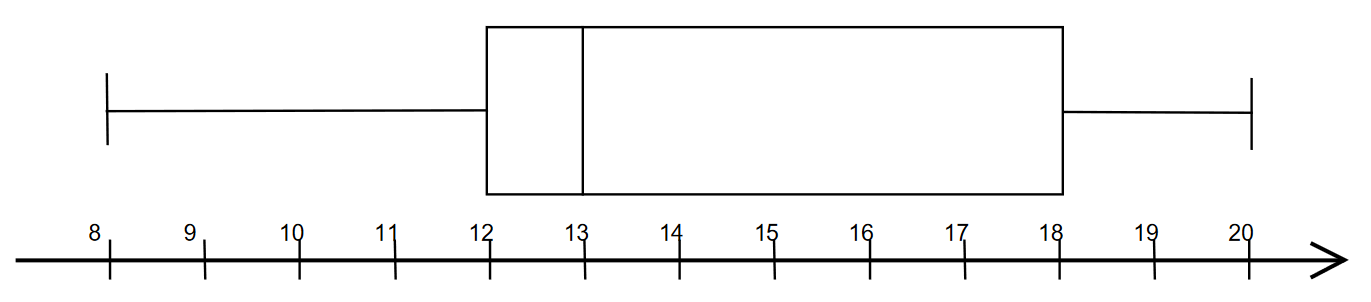
\includegraphics[scale=0.4]{boite2}
	\end{center} 
	
	\fillwithdottedlines{5cm}
	
\end{questions}